\documentclass{school}

\title{Statistik}
\subject{Angewandte Mathematik}
\author{Markus Reichl}

\begin{document}
\maketitle
\thispagestyle{fancy}	% Makes the first page fancy too

\tableofcontents

\section{Statistik}
\subsection{Begriffe}
\begin{tabularx}{\textwidth}{X c l}
Mittelwert & $\bar{x} = \frac{Summe}{Anzahl}$ & \small{Durchschnittlicher Wert einer Liste.}\\
Standardabweichung & $\sigma = \sqrt{\frac{1}{n} \sum_{i=1}^{n} (x_i - \bar{x})^2}$ & \small{Mittlere Abweichung vom Mittelwert.}\\
Varianz & $\sigma^2$ & \small{Mittlere quadratische Abweichung vom Mittelwert.}\\
Median & $\hat{x}$ & \small{Mittlerer Wert einer geordneten Liste.}\\
Minimum & $x_0$ & \small{Erster Wert einer geordneten Liste.}\\
Maximum & $x_n$ & \small{Letzter Wert einer geordneten Liste.}\\
Spannweite & $r = x_0 - x_n$ & \small{Differenz zwischen Minimum und Maximum.}\\
1. Quartil & $q_1$ & \small{Median der Werte vor dem Median einer geordneten Liste.}\\
2. Quartil & $q_2 = \hat{x}$ & \small{Median einer geordneten Liste.}\\
3. Quartil & $q_3$ & \small{Median der Werte nach dem Median einer geordneten Liste.}
\end{tabularx}

\newpage
\subsection{Darstellung}
\subsubsection{Boxplot}
Aus dem Boxplot lassen sich die Quartile, der Median, sowie Minimum und Maximum auslesen. Dabei wird eine Skala vom Minimum zum Maximum gezogen und eine Box vom 1. bis zum 3. Quartil gespannt, die vom Median geteilt wird. Zusätzlich können auch Ausreißer vor oder nach dem Boxplot gezeichnet werden.
\begin{figure}[h]
	\centering
	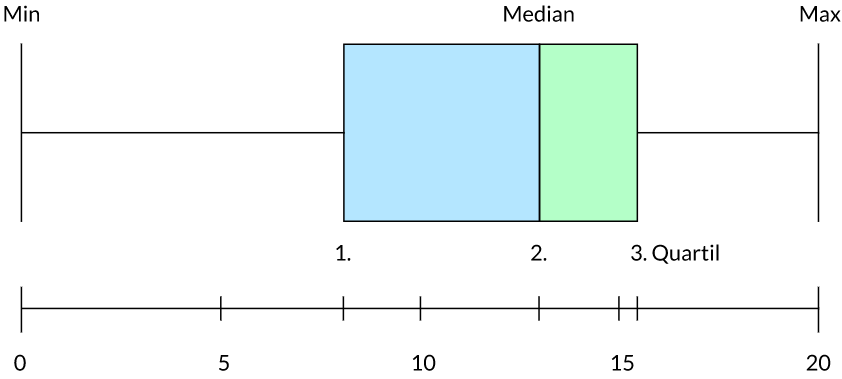
\includegraphics[width=0.5\textwidth]{boxplot.png}
	\caption{Boxplot}
\end{figure}

In wxMaxima kann ein Boxplot mittels \verb|wxboxplot(<<liste>>, box_orientation=horizontal)| dargestellt werden.

\subsubsection{Kreisdiagramm}
\subsubsection{Histogramm}
\paragraph{Absolute Häufigkeit}
\paragraph{Relative Häufigkeit} 

% Basic Figure
% \begin{figure}[h]
%	 \centering
% 	 \includegraphics[height=4cm]{image.jpg}
% 	 \caption{Caption}
% \end{figure}

% Basic bibiography
% \begin{thebibliography}{9}
% \bibitem{faz} faz.net, Vergewaltigung live auf Facebook gezeigt \\ http://www.faz.net/aktuell/gesellschaft/kriminalitaet/vergewaltigung-live-auf-facebook-gezeigt-14936872.html
% \end{thebibliography}

% List of figures
% \listoffigures
\end{document}